\documentclass{beamer}
\usepackage{beamerthemesplit}
\usepackage{pgfgantt}
\usetheme{Warsaw}
\usecolortheme{wolverine}
\usepackage{sidecap}
%\usepackage[frenchb]{babel}
%\usepackage[latin1]{inputenc}
\usepackage[utf8x]{inputenc}
\usetikzlibrary{babel}
\usepackage[T1]{fontenc}
\usepackage{amsfonts}
\usepackage{amsmath,amssymb,theorem}
\usepackage[all]{xy}
\usepackage{textcomp}
\usepackage{pstricks,pst-plot,pstricks-add}
\usepackage{bm, listings, ccaption}
\usepackage{xcolor,epic,eepic,multicol, colortbl}
\graphicspath{{Images_Fichiers/}}
\lstset{language=C++,
                basicstyle=\ttfamily,
                keywordstyle=\color{blue}\ttfamily,
                stringstyle=\color{red}\ttfamily,
                commentstyle=\color{green}\ttfamily,
                morecomment=[l][\color{magenta}]{\#}
}
\newcommand{\gs}[1]{\textbf{\underline{#1}}}
\newcommand{\R}{\mathbb{R}}
 
\graphicspath{{Images/}}
\title{UE Projet Altran 2020-2021}
\author{GRAFF Jonathan}
\date{\today}
\begin{document}
\maketitle
\tableofcontents
\section{Introduction - Contexte } 
\begin{frame}
\frametitle{Introduction - Contexte}
Altran : \begin{itemize}
\item conseil
\item ingénierie
\item recherche et développement
\pause
\item domaine : Automobile, Aéronautique, Spatial, Transport, Energie, Industrie, Communications, Electronique, Logiciel, Internet, Finance, Secteur Public \dots
\pause
\item 30 pays, 50000 employés
\end{itemize}
\end{frame}

\begin{frame}
Le projet : 

Altran Research \pause$\rightarrow$ Future of Energy \pause $\rightarrow$  Sinbad \pause $\rightarrow$ Anagreen\medskip

Anagreen : collaboration avec ArcelorMittal, financé par l'ADEME (Agence de l'environnement et de la maîtrise de l'énergie)\medskip

Le but : développer un outil d'aide à la décision pour la récupération de la chaleur fatale dans l'industrie
\end{frame}
\section{Problèmes des réseaux d'échangeur thermiques}
\subsection{Motivation}
\begin{frame}
La chaleur fatale : chaleur résiduelle issue d'un procédé et non utilisée par celui-ci.
\pause
\begin{itemize}
\item 16 \% de la consommation énergétique nationale

\pause 

\item 36\% de la consommation industrielle

\pause 

\item probablement sous-évalué\pause

\end{itemize}

Historiquement : \begin{itemize}
\item peu d'intérêt jusqu'aux années 1970 (énergie peu chère, peu de conscience écologique)\pause

\item prise de conscience aujourd'hui (énergie plus chère, taxes sur les rejets polluants...) d'où l'intérêt des entreprises
\end{itemize}


\end{frame}
\subsection{Généralités sur les échangeurs thermiques}
\begin{frame}
Un échangeur thermique est un dispositif permettant
de transférer de la chaleur d'un flux chaud vers un flux plus froid, sans les mélanger

Trois types : \begin{itemize}
\item à co-courant \pause
\item à contre-courant \pause
\item à courant croisés
\end{itemize}

\end{frame}
\begin{frame}

Plusieurs montages différents :  

{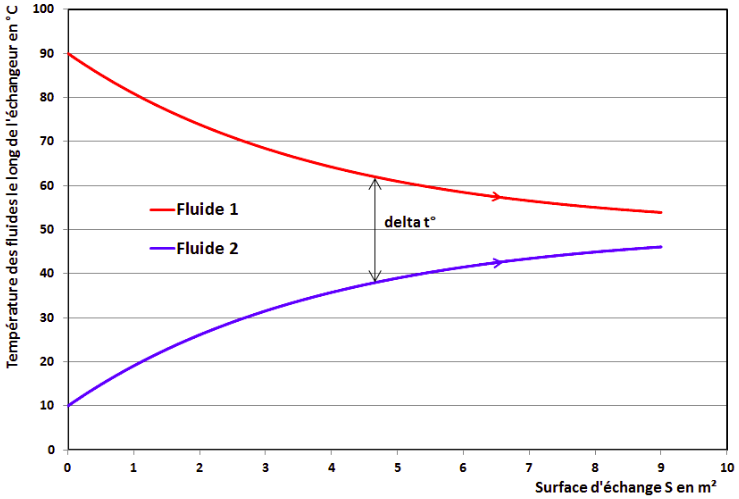
\includegraphics[scale=0.4]{1.png}}

\end{frame}
\begin{frame}

Plusieurs montages différents :  

{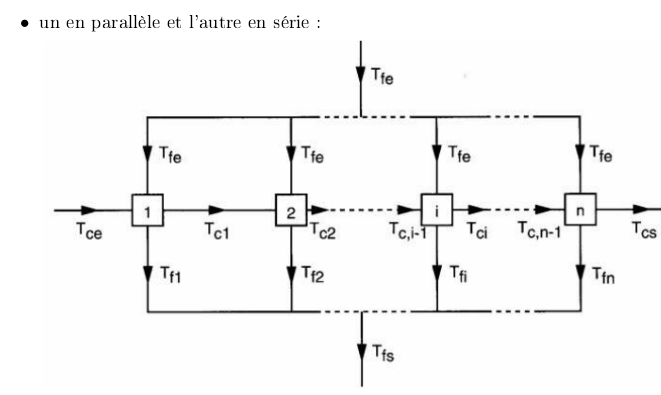
\includegraphics[scale=0.4]{2.png}}

\end{frame}
\begin{frame}

Plusieurs montages différents :  
en maillage :

{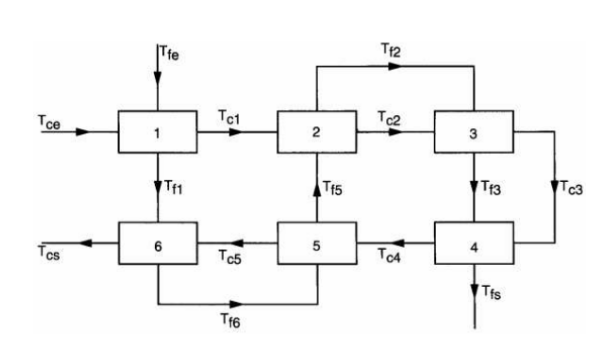
\includegraphics[scale=0.4]{3.png}}

\end{frame}

\begin{frame}

Plusieurs montages différents :  \bigskip

Les deux en parallèle. Cette méthode est moins utilisée que les autres pour des raisons de
performances moindres.

\end{frame}

\subsection{Réseaux d'échangeurs thermiques}

\begin{frame}
\begin{itemize}
\item flux chauds - flux froids \pause
\item Quels échangeurs placer ?\pause
\item Où les placer ?\pause
\item Quand les placer ?\pause
\end{itemize}
Le problème est combinatoire : problème NP-difficile !\pause

Pour 10 flux chauds et 10 flux froids, si on se limite à 15 échangeurs, il y a $3\times 10^{24}$ possibilités différentes, juste pour le placement.
\end{frame}

\subsection{Etat de l'art}
\begin{frame}
Plusieurs solutions apportées pour ces problèmes : 

\begin{itemize}
\item méthode empirique : repose sur des avis d'experts \pause
\item méthode du pincement : consiste à diviser le problème en deux sous-problèmes plus simples. Repose sur des principes thermodynamiques \pause
\item algorithmes mathématiques : gloutons, programmation linéaire ou non linéaire mixte entière, génétiques, stochastiques, recuit simulé... \pause


\end{itemize}
Toutes ces solutions ont des avantages et des inconvénients, mais aucune n'est assurée de donner a solution optimale
\end{frame}

\section{Nouvelle solution : l'apprentissage par renforcement profond}

\begin{frame}
\frametitle{Nouvelle solution : l'apprentissage par renforcement profond}
Le but du projet ici est de vérifier si une méthode par apprentissage par
réseaux de neurones à renforcement profond, pourrait résoudre ce problème d'optimisation combinatoire.\pause \medskip

L'idée vient de l'équipe de Google Brain qui a obtenu des résultats encourageants sur le problème du voyageur de commerce.
\pause \medskip

Le but du projet Anagreen est de se demander si ces mêmes résultats pourraient être transposables sur ce problème
de réseaux d'échangeurs de chaleur.
\end{frame}

\begin{frame}

\frametitle{Le principe}
L'apprentissage par renforcement : \medskip

Un agent (robot) apprend par lui-même le comportement à adopter face à un problème à résoudre. L'agent est placé dans un environnement et peut avoir plusieurs états. Par rapport à chaque état, il peut effectuer un ensemble d'actions. \pause
\begin{center}

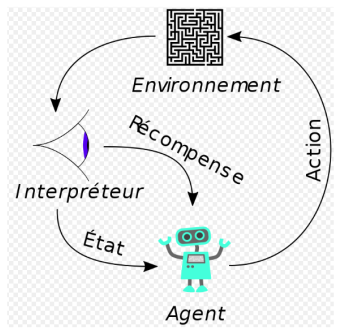
\includegraphics[scale=0.38]{4.png}
\end{center}
\end{frame}

\begin{frame}
\frametitle{Le principe :}
\begin{itemize}
\item L'agent choisit son action (ou reçoit les probabilités d'action) selon une fonction appelée "politique".\pause
\item A chaque action effectuée, l'agent va changer d'état, et recevoir une récompense.\pause
\end{itemize}
Pendant la phase d'apprentissage,
l'agent va alterner entre deux comportements :\pause
\begin{itemize}
\item une phase d'exploration où l'agent va tester aléatoirement de nouvelles actions\pause
\item une phase d'exploitation, où la politique actuelle est éprouvée.\pause
\end{itemize}
Les états terminaux : le jeu s'arrête (gagné ou perdu)
\end{frame}

\begin{frame}
L'environnement renvoie à l'agent, en fonction de son état $s$ et de son action $a$, un autre état $s'$ et une récompense $r$, qui est un nombre réel. Mathématiquement, $env$ est une fonction $$env :\begin{array}[t]{lcr}
S\times A &\rightarrow& S \times \R\\
(s,a) & \mapsto & (s', r)\\\end{array}$$\medskip \pause

Le but est de trouver une suite de paires état-action $(s,a)$ qui maximise la récompense $G$, où $G$ vérifie :
$$G = \sum_{t} \gamma ^t r_t$$\pause
$\gamma$ est le facteur de réduction : sert à faire converger la somme et à rendre les récompenses immédiates plus importantes (en général $\approx 0.9$).
\end{frame}

\begin{frame}
\frametitle{La Q-fonction optimale}
$$
Q^{*}(s,a) := \max_{ (s_t,a_t)\ _{t\geq 0}}\left( \sum_{t\geq 0} \gamma^t r_t  \ \big | s_0=s,a_0=a\right)
$$
\pause
La fonction $Q^{*}$ est appelée la $Q$-fonction optimale. Il s'agit de la fonction qui renvoie la récompense maximale pouvant être obtenue à partir d'un état et d'une action de départ. \pause

La fonction n'est pas connue, on va chercher à l'approcher. 

Une fois cette fonction connue, on connaitra aussi la trajectoire à suivre pour obtenir ce maximum :

$$
a_1 = \text{argmax}_{a\in A_{s_1}} Q^{*}(s_1,a), ~ a_2 = \text{argmax}_{a\in A_{s_2}} Q^{*}(s_2,a) \text{ etc}.
$$
\end{frame}

\subsubsection{Théorème de Bellmann}
\begin{frame}
\frametitle{Théorème de Bellmann}
Soient $(s,a)$ un couple état-action, et posons $(s',r)= env(s,a)$.  La fonction $Q^{*}$ vérifie:   
$$
Q^{*}(s,a) = r + \gamma \max_{a'\in A_{s'}} Q^{*}(s',a')
$$\pause

Approcher la fonction $Q^*$ par un algorithme itératif. 

Si $Q$ vérifie "à peu près" la relation précédente, alors $Q$ sera proche de $Q^*$. 
\end{frame}

\subsubsection{Algorithme du $Q$-learning}
\begin{frame}
\frametitle{L'algorithme}
\vspace*{-0.3cm}
\begin{enumerate}
\item on initialise $Q$ à $0$, $\epsilon$ à $1$\pause

\item on choisit un état $s$ aléatoirement\pause

\item on choisit aléatoirement une action avec une probabilité de $\epsilon$ : c'est la phase d'\textbf{exploration}.\\ Et avec une probabilité de $1-\epsilon$, on choisit l'action qui maximise $Q(s,a)$ (avec le $Q$ courant) : c'est la phase d'\textbf{exploitation}.\pause

\item on calcule $s', r = env(s, a)$ et on met à jour : $$ 
Q(s,a) = r + \gamma \max_{a'} Q(s',a')$$

\item on diminue $\epsilon$.\pause

\item si l'état $s$ n'est pas terminal, on recommence à l'étape 3 avec $s=s'$. S'il l'est, on recommence à l'étape 2. \pause

\item On arrête l'algorithme selon un critère d'arrêt, par exemple au bout d'un nombre fixé d'itérations

\end{enumerate} 
\end{frame}

\subsection{Apprentissage par renforcement profond}
\begin{frame}
\frametitle{Apprentissage par renforcement profond}
Le nombre d'états est en général immense, souvent même infini $\Rightarrow$ impossible de construire la fonction $Q$\pause \medskip

On utilise alors à la place un réseaux de neurones pour pouvoir prédire la valeur de la fonction $Q$, en général un réseau de neurones à plusieurs couches cachées, d'où le nom "profond".\pause \medskip

En pratique, on part d'un couple état-action initial $(s,a)$, et on construit un batch d'états-action en suivant la même stratégie que précédemment, selon $\epsilon$. \pause \medskip

Une fois ce batch construit, on l'utilise pour modifier les poids $\omega$ du réseau de façon à ce que la distance entre les $
Q(s,a) \text{ et les } r + \gamma \max_{a'} Q(s',a')$ soit minimale (où $s'$ est l'état renvoyé après l'action $a$).


\end{frame}

\section[Implémentation d'un exemple]{Implémentation d'un exemple}
\subsubsection[L'environnement]{L'environnement}

\begin{frame}
\frametitle{Implémentation d'un exemple : GridWorld}
L'environnement sera une grille :
\begin{itemize}
\item l'agent en haut à gauche : $(0,0)$
\item en-bas à droite : un trésor
\item au-dessus : une bombe
\item des obstacles
\end{itemize}
Les états terminaux : la bombe et le trésor.
\end{frame} 

\begin{frame}
$$\begin{array}{|c|c|c|c|c|}
\hline
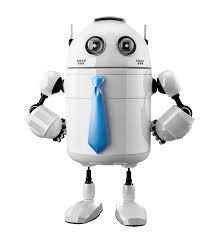
\includegraphics[scale=0.15]{agent.jpeg} & \hspace*{1cm} &  \hspace*{1cm}&  \hspace*{1cm} & \\
\hline
& & \cellcolor{black} & & \\
& & \cellcolor{black} & & \\
\hline
& \cellcolor{black} & & & 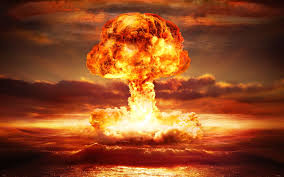
\includegraphics[scale=0.15]{bombe.jpeg}\\
\hline
& & & & 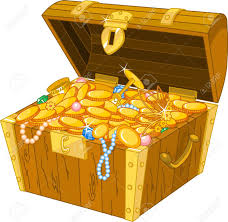
\includegraphics[scale=0.15]{tresor.jpeg} \\
\hline
\end{array}
$$
\end{frame}

\begin{frame}
\frametitle{Les actions}
Il y a quatre actions possibles
\begin{itemize}
\item haut
\item gauche
\item droite
\item haut
\end{itemize}\pause

Si il y a un bord ou un obstacle, l'agent reste au même endroit. 




\end{frame}

\begin{frame}
\frametitle{Les récompenses}
\begin{itemize}
\item +10 pour un déplacement sur le trésor
\item -10 pour un déplacement sur la bombe
\item -1 pour chaque déplacement
\end{itemize}
\pause
\centering
$$\begin{array}{|c|c|c|c|c|}
\hline
-1 & -1 & -1 & -1 & -1 \\
\hline
-1 & -1 & 0 & -1 & -1 \\
\hline
-1 & 0 & -1 & -1 & -10 \\
\hline
-1 & -1 & -1 & -1 & 10 \\
\hline
\end{array}
$$
\end{frame}

\begin{frame}
\frametitle{Les résultats}
Un agent aléatoire et un agent apprenant

\begin{figure}[!ht]
\hspace*{0cm}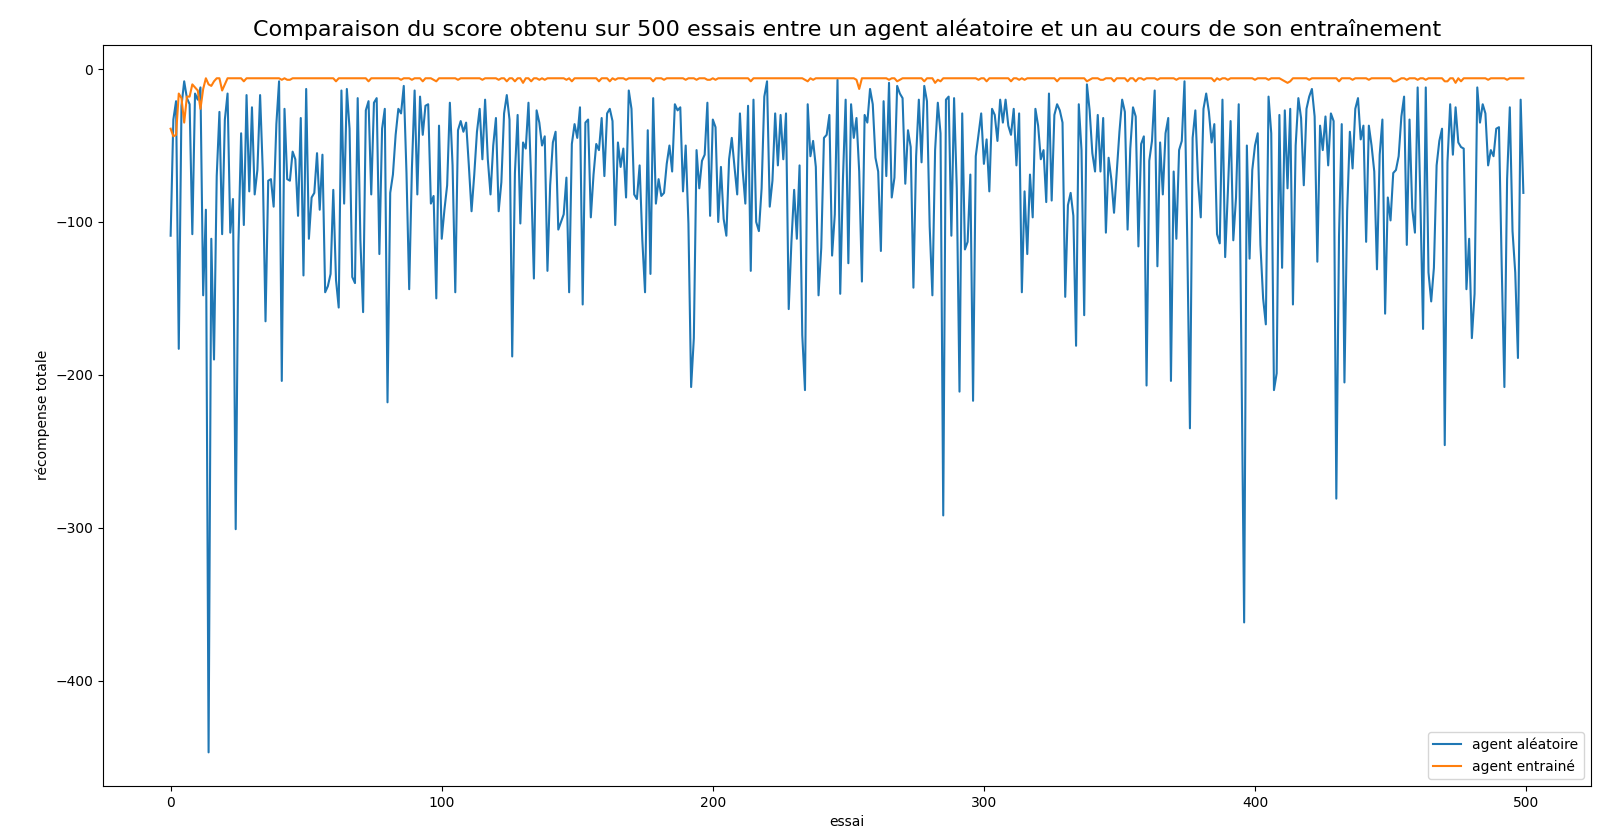
\includegraphics[scale=0.20]{resultats.png}
\end{figure}


L'agent qui apprend est très vite beaucoup plus efficace que l'agent aléatoire 
\end{frame}

\begin{frame}
\frametitle{Les résultats}
\begin{figure}[!ht]
\hspace*{0cm}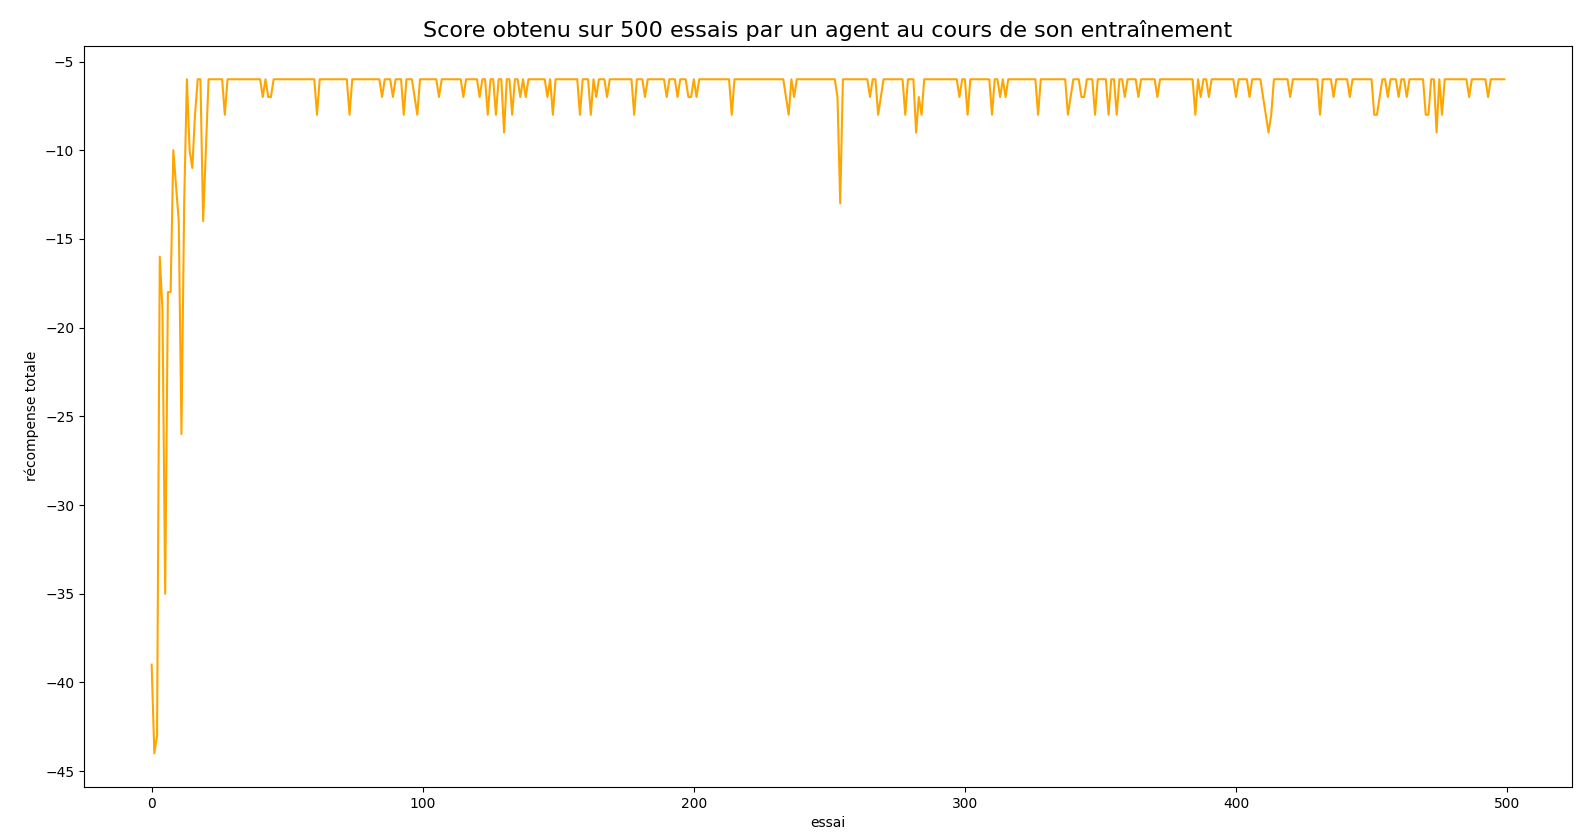
\includegraphics[scale=0.21]{resultats2.png}
\label{recompgraph2}
\end{figure}
On voit bien que les résultats varient beaucoup au début, puis de moins en moins au fur et à mesure de l'apprentissage de l'agent. 
\end{frame}

\begin{frame}
\frametitle{La Q-table}

La Q-table est composée, pour chaque case de la grille, d'un dictionnaire. 
\begin{itemize}
\item Ses quatre clés sont les quatre actions
\item Ses valeurs sont celles de Q(état, action)
\end{itemize}
Voici une représentation dans une grille $3 \times 3$ : 
\end{frame}

\begin{frame}
\begin{figure}[!ht]
\centering
$$\begin{array}{|c|c|c|}
\hline
0                      & 0                           & 0 \\
0\hspace*{0.25cm}\textcolor{red}{A}\hspace*{0.25cm} 0 & 0\hspace*{0.8cm} 0                  & 0\hspace*{0.6cm}0 \\
0          & 0          & 0 \\
\hline
0          & 0                            & 0 \\
0\hspace*{0.6cm}0   & 0\hspace*{0.6cm} 0                  & 0\hspace*{0.25cm}\textcolor{red}{B}\hspace*{0.25cm} 0 \\
0           & 0          & 0 \\
\hline
0          & 0                         & 0\\
0\hspace*{0.6cm} 0                     & 0\hspace*{0.6cm}0                & 0\hspace*{0.25cm}\textcolor{red}{T}\hspace*{0.25cm} 0 \\
0                            & 0        & 0 \\
\hline
\end{array}
$$
\end{figure}
\end{frame}

\begin{frame}
Si l'agent va à droite, il recevra une récompense de $-1$. Donc : 
$$Q((0,0), "droite") = -1 + \max_{a'} Q((0,1), a') = -1+0 = -1$$
\end{frame}

\begin{frame}
\begin{figure}[!ht]
\centering
$$\begin{array}{|c|c|c|}
\hline
0                      & 0                           & 0 \\
0\hspace*{0.8cm} -1 & 0\hspace*{0.25cm}\textcolor{red}{A}\hspace*{0.25cm}  0                  & 0\hspace*{0.6cm}0 \\
0          & 0          & 0 \\
\hline
0          & 0                            & 0 \\
0\hspace*{0.6cm}0   & 0\hspace*{0.6cm} 0                  & 0\hspace*{0.25cm}\textcolor{red}{B}\hspace*{0.25cm} 0 \\
0           & 0          & 0 \\
\hline
0          & 0                         & 0\\
0\hspace*{0.6cm} 0                     & 0\hspace*{0.6cm}0                & 0\hspace*{0.25cm}\textcolor{red}{T}\hspace*{0.25cm} 0 \\
0                            & 0        & 0 \\
\hline
\end{array}
$$
\end{figure}
\end{frame}

\begin{frame}
Si l'agent va ensuite à droite et en-bas, il recevra à chaque fois une récompense de $-1$. A la fin du premier épisode, on aura donc : \pause
\begin{figure}[!ht]
\centering
$$\begin{array}{|c|c|c|}
\hline
0                      & 0                           & 0 \\
0 -1 & 0 \hspace*{0.6cm} -1 & 0\hspace*{0.6cm}0 \\
0          & 0          & -10 \\
\hline
0          & 0                            & 0 \\
0\hspace*{0.6cm}0   & 0\hspace*{0.6cm} 0                  & 0\hspace*{0.25cm}\textcolor{red}{B A}\hspace*{0.25cm} 0 \\
0           & 0          & 0 \\
\hline
0          & 0                         & 0\\
0\hspace*{0.6cm} 0                     & 0\hspace*{0.6cm}0                & 0\hspace*{0.25cm}\textcolor{red}{T}\hspace*{0.25cm} 0 \\
0                            & 0        & 0 \\
\hline
\end{array}
$$
\end{figure}

\end{frame}
\begin{frame}
Imaginons un deuxième épisode où le chemin choisi sera $$\text{"droite - bas - bas - droite"}$$ 

Alors : \pause

\begin{figure}[!ht]
\centering
$$\begin{array}{|c|c|c|}
\hline
0                      & 0                           & 0 \\
0 -1 & 0 \hspace*{0.6cm} -1 & 0\hspace*{0.6cm}0 \\
0          & -1          & -10 \\
\hline
0          & 0                            & 0 \\
0\hspace*{0.6cm}0   & 0\hspace*{0.6cm} 0                  & 0\hspace*{0.25cm}\textcolor{red}{B}\hspace*{0.25cm} 0 \\
0           & -1          & 0 \\
\hline
0          & 0                         & 0\\
0\hspace*{0.6cm} 0                     & 0\hspace*{0.6cm}10                & 0\hspace*{0.25cm}\textcolor{red}{T A}\hspace*{0.25cm} 0 \\
0                            & 0        & 0 \\
\hline
\end{array}
$$
\end{figure}
\end{frame}

\begin{frame}
Si à un troisième épisode, le chemin choisi est $$\text{"bas - droite - bas - droite"}$$ 
\pause
\begin{figure}[!ht]
\centering
$$\begin{array}{|c|c|c|}
\hline
0                      & 0                           & 0 \\
0 -1 & 0 \hspace*{0.6cm} -1 & 0\hspace*{0.6cm}0 \\
-1          & -1          & -10 \\
\hline
0          & 0                            & 0 \\
0\hspace*{0.6cm}-1   & 0\hspace*{0.6cm} 0                  & 0\hspace*{0.25cm}\textcolor{red}{B}\hspace*{0.25cm} 0 \\
0           & 9         & 0 \\
\hline
0          & 0                         & 0\\
0\hspace*{0.6cm} 0                     & 0\hspace*{0.6cm}10                & 0\hspace*{0.25cm}\textcolor{red}{T A}\hspace*{0.25cm} 0 \\
0                            & 0        & 0 \\
\hline
\end{array}
$$
\end{figure}
\end{frame}

\begin{frame}
Avec deux autres épisodes on obtiendra donc la Q-table suivante : \pause

\begin{figure}[!ht]
\centering
$$\begin{array}{|c|c|c|}
\hline
0                      & 0                           & 0 \\
0 -1 & 0 \hspace*{0.6cm} -1 & 0\hspace*{0.6cm}0 \\
7          & -1          & -10 \\
\hline
0          & 0                            & 0 \\
0\hspace*{0.6cm}8   & 0\hspace*{0.6cm} 0                  & 0\hspace*{0.25cm}\textcolor{red}{B}\hspace*{0.25cm} 0 \\
0           & 9         & 0 \\
\hline
0          & 0                         & 0\\
0\hspace*{0.6cm} 0                     & 0\hspace*{0.6cm}10                & 0\hspace*{0.25cm}\textcolor{red}{T A}\hspace*{0.25cm} 0 \\
0                            & 0        & 0 \\
\hline
\end{array}
$$
\end{figure}
\end{frame}

\begin{frame}
\frametitle{Les résultats pour la grille $5\times 3$}
\hspace*{-0.95cm}$\begin{array}{|c|c|c|c|c|}
\hline
-2.02                           & 0.60                          & 2.11                           & 1.41                           & -0.8 \\
-1.07~ ~ \textcolor{red}{4.00}  & 0.55~ ~ \textcolor{red}{5.00} & -0.57~ ~ \textcolor{red}{6.00} & 1.71~ ~ -1.21                  & -0.80~ ~ -0.80 \\
-3.30                           & -2.59                         & 0.60                           & \textcolor{red}{7.00}          & \textcolor{red}{-0.10} \\
\hline
-2.56                         & \textcolor{red}{1.29}        & 0.00           & 4.07                            & -0.46 \\
-2.60~ ~ -2.54                & 2.51~ ~-2.57                 & 0.00~ ~ 0.00   & 6.46~ ~ -0.40                   & \textcolor{red}{3.46}~ ~ -0.50 \\
\textcolor{red}{-2.48}        & -2.58                        & 0.00           & \textcolor{red}{8.00}          & -0.47 \\
\hline
-1.78                          & 0.00          & -0.10          & 1.56                         & 0.00\\
-1.80~ ~ -1.80                 & 0.00~ ~ 0.00  & 0.04~ ~ \textcolor{red}{5.14}                     & 1.35~ ~ -4.69                & 0.00~ ~ 0.00 \\
\textcolor{red}{-1.20}         & 0.00          & -0.10                            & \textcolor{red}{9.00}        & 0.00 \\
\hline
-1.20                              & -0.59                          & -0.10                           &  6.28                           & 0.00 \\
-1.12~ ~ \textcolor{red}{1.03}     & -0.56~ ~ \textcolor{red}{4.31} & -0.34~ ~ \textcolor{red}{8.13}  &  2.25~ ~ \textcolor{red}{10.00} & 0.00~ ~ 0.00 \\
-1.10                              & -0.60                          & -0.10                           & 4.70                           & 0.00 \\
\hline
\end{array}
$
\end{frame}

\frame{
\centering\textbf{\LARGE Merci pour votre attention !}

}

\end{document}
